\section{L'importanza dell'apprendimento}

Le reti neurali~\cite{ann} sono alla base del deep learning, che è un sottocampo del machine learning.
Questa ultima branca è fondamentale nello studio e nello sviluppo delle Intelligenze Artificiali, sistemi basati sull’apprendimento automatico partendo dallo studiare i dati in input per fornire dati più vicini possibile a quelli desiderati. 
Sostanzialmente un algoritmo di machine learning è un algoritmo capace di apprendere dai dati. \\

\emph{"Si dice che un programma apprende dall'esperienza E con riferimento a alcune classi di
 compiti T e con misurazione della performance P, se le sue performance nel compito T, come misurato da P,
  migliorano con l'esperienza E."}~\cite{learning}

Tom M. Mitchell\footnote{Tom Michael Mitchell è un computer scientist americano e professore universitario. 
É conosciuto per aver contribuito attivamente allo sviluppo degli studi sul machine learning e le intelligenze artificiali.} \\

Il compito principale del machine learning è che una macchina sia in grado di generalizzare
 dalla propria esperienza. Per generalizzazione si intende l'abilità di una macchina di portare a
  termine in maniera accurata esempi o compiti nuovi, che non ha mai affrontato, 
  dopo aver fatto esperienza su un insieme di dati di apprendimento.\\
La macchina ha il compito di costruire un modello probabilistico generale dello spazio delle 
occorrenze di un determinato fenomeno da apprendere tramite dei \emph{training examples}, in maniera 
tale da essere in grado di produrre previsioni sufficientemente accurate quando sottoposta a nuovi casi. 
Proprio a questo proposito, al fine di valutare la bontà di un algoritmo di machine learning,
 dobbiamo stimare un andamento qualitativo della sua performance P, la quale molto spesso è specifica 
 per un determinato compito T che il sistema deve compiere. 

I compiti dell'apprendimento automatico vengono tipicamente classificati in tre ampie categorie, 
sulla base dell’esperienza E a cui sono sottoposti nel processo di apprendimento, dunque a seconda 
della natura del "segnale" utilizzato per l'apprendimento o del "feedback" disponibile al sistema di
 apprendimento. Queste categorie, anche dette paradigmi, sono~\cite{ml}:
 \begin{itemize}
\item \textbf{apprendimento supervisionato}, in cui al modello vengono forniti degli esempi nella forma
 di possibili input e output desiderati e l'obiettivo è quello di estrarre una regola
  generale che associ l'input all'output corretto;
\item \textbf{apprendimento non supervisionato}, in cui il modello ha lo scopo di trovare una
 struttura negli 
input forniti, senza che questi vengano etichettati in alcun modo;
\item \textbf{apprendimento per rinforzo}, il quale punta a realizzare agenti 
autonomi in grado di scegliere
 azioni da compiere per il conseguimento di determinati obiettivi tramite interazione con l'ambiente
  in cui sono immersi. 
\end{itemize}
Il tipo di apprendimento di interesse per il lavoro di tesi è quello supervisionato, in quanto si utilizzano coppie input-output 
rappresentate da immagini e label che le identificano. \\
Tra i compiti più importanti dell’apprendimento supervisionato vi sono la classificazione
 e la regressione, i quali si distinguono a seconda di come viene considerato l’output 
 del sistema di apprendimento. 
 Nella prima gli output sono divisi in due o più classi e il sistema di apprendimento 
 deve produrre un modello che assegni gli input non ancora visti a una o più di queste~\cite{class}. 
 Si dice che i valori assunti dall'ouput sono \emph{qualitativi}. 
 Nella seconda invece si può dire che a differenza della prima i dati in output sono continui, 
 cioè non riguardano una categorizzazione: si dice che i valori assunti dall'output sono \emph{quantitativi},
  in quanto restituiscono la stima di una misura. \\
La classificazione è il compito su cui verte il presente lavoro di tesi.
 Per tale scopo, la performance P dell’algoritmo di machine learning si valuta misurando
  l’accuratezza del modello cioè la percentuale di esempi per i quali il modello elabora
   un output 
  corretto sul totale delle osservazioni. Un altro parametro di riferimento può essere il
   rate di errore,
   definito invece come la
    proporzione di esempi per cui il sistema elabora un output sbagliato.


É importante verificare come l’algoritmo riesca a valutare dati che non abbia mai visto.
 Misure di performance vengono effettuate usando un insieme di dati chiamato insieme di \emph{test}.
  Questo insieme di dati è di solito diverso dall’insieme di esempi usati per allenare 
  il sistema (insieme di \emph{addestramento} o \emph{training}) affinchè si possano
   fare valutazioni
   più precise ed indipendenti da quanto sia stato efficace l’addestramento.
Di solito l’esperienza E corrisponde ad un intero \emph{dataset}, una collezione di dati
 (che possono essere sotto forma di vettori, immagini, suoni ecc.) 
 suddiviso in classi tale per cui ad ogni elemento è associata una ed una sola di queste. 
 Tali dati, essendo utilizzati
  in fase di addestramento, è estremamente importante che siano costruito in maniera corretta.
  Dunque il punto di partenza per un buon addestramento è sicuramente un buon dataset.
 \\
 
Come accennato sopra, l’apprendimento supervisionato è una forma di apprendimento automatico
 in cui al sistema da allenare si sottopone in input un insieme di addestramento formato 
 da esempi
  etichettati con il rispettivo valore di output desiderato, e tra gli input e output
   si vuol trovare una corrispondenza.
   Questo processo fa tipicamente 
  riferimento a tecniche
  di tipo statistico. \\
L'apprendimento consiste nell’osservazione di una quantità di esempi di un vettore casuale 
\textbf{x} a cui è associato un vettore \textbf{y}  per poi apprendere come predire \textbf{y} 
da \textbf{x}~\cite{prob}, 
stimando una distribuzione
 di probabilità condizionata\footnote{Date due variabili aleatorie X e Y,
  la distribuzione condizionata di Y dato X è la probabilità di Y quando è conosciuto il valore 
  assunto da X.} p(\textbf{y}$\mid$\textbf{x}) per l'output, che consenta di ottenere 
  anche buoni valori di 
 confidenza per l'algoritmo. \\
 I valori di \textbf{y} fungono da guida per indirizzare e migliorare 
 l’apprendimento di contro al caso non supervisionato in cui l’algoritmo deve trattare i dati 
 senza l’ausilio di questa guida. \\
Un esempio di apprendimento supervisionato è  il training di un sistema
col compito di riconoscimento delle immagini.
In questo caso dobbiamo specificare quale oggetto appare in ogni foto.
Possiamo fare questo con un codice numerico che caratterizzi le varie classi, per esempio
usando 0 per le persone, 1 per le macchine, 2 per i gatti, e così via, a seconda di quello che
 è l'elemento di interesse da riconoscere.\\
 \begin{figure}[H]
  \centering
  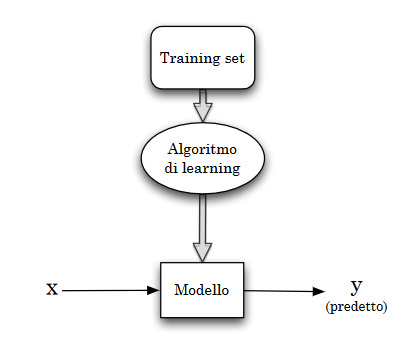
\includegraphics[width=0.8\textwidth]{Figures/schema apprendimento supervisionato.png}
  \caption{\small{Schema dell' apprendimento supervisionato~\cite{img_learning}. 
  } % end small
  } % end caption
  \label{fi:dcalc}
\end{figure}

\section{Neuroni artificiali e deep learning}

Le \emph{reti neurali}~\cite{reti} si riferiscono storicamente alla rete di neuroni che si trovano nel cervello dei mammiferi,
 e la loro struttura ne ha ispirato gli algoritmi. I neuroni sono le unità fondamentali di calcolo, 
 e sono connessi tra loro in reti per processare dati. Essi rispondono a stimoli esterni, così come 
 le reti neurali prendono dati in input, si allenano nel riconoscere dei pattern ripetuti all’interno 
 dei dati, e sono in grado di predire l’output per un set di dati simili.\\
  La corteccia cerebrale umana
  contiene circa 1010 neuroni. Sono collegati tra loro da filamenti nervosi (assoni) che si diramano e
   terminano in sinapsi, connessioni verso altri neuroni. Le sinapsi connettono verso i dendriti, 
   diramazioni che si estendono dal corpo della cellula neurale e sono atti a ricevere impulsi da 
   altri neuroni nella forma di segnali elettrici. Nelle reti neurali biologiche lo spessore dei 
   dendriti definisce il peso ad esso associato. La rete risultante di neuroni tra loro connessi 
   nella corteccia cerebrale è responsabile del processare immagini, audio e dati sensoriali. 
   In presenza di una differenza di potenziale fra esterno e l’interno della cellula, il neurone 
   si attiva trasmettendo un impulso elettrico attraverso il suo assone che provoca la liberazione
    di un neurotrasmettitore.\\
Nelle reti neurali artificiali, il modo in cui le informazioni sono processate e i segnali 
sono trasferiti sono ampiamente idealizzati da tali concetti. \\
\begin{figure}[hb!]
  \centering
  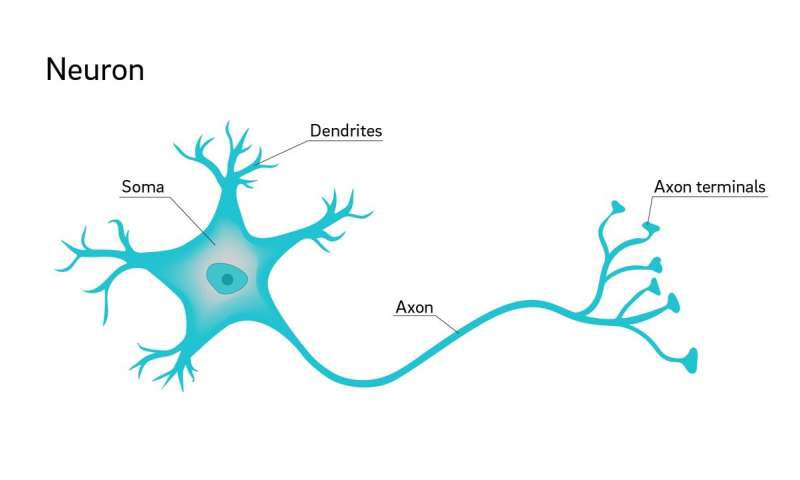
\includegraphics[width=1\textwidth]{Figures/neuron.jpeg}
  \caption{\small{Un semplice schema di neurone. ~\cite{neuron}
   } % end small
  } % end caption
  \label{fi:dcalc}
\end{figure}

 Il primo modello computazionale di neurone è stato proposto nel 1943 da Warren MuCulloch
  e Walter Pitts \footnote{McCulloch e Pitts sono stati un neurofisiologo e un logico americani famosi per essere stati i primi a realizzare il primo modello matematico di rete neurale}. 
McCulloch and Pitts hanno pensato ad un modello di neurone come un’unità di \emph{threshold} (soglia) binaria.

Essa possiede due possibili stati: attivo o inattivo.\\
  Per ottenere il segnale di output il neurone elabora una 
 somma pesata degli input: se la somma eccede un certo valore di threshold, lo stato del neurone
  risulta attivo, altrimenti inattivo.
Il modello, in intervalli discreti di tempo t = 0, 1, 2, 3… , svolge del calcolo computazionale. \\
Lo stato del neurone numero j al passo t è identificato come:

\[s_j(t) = \left\{\begin{matrix}
    1 & \text{attivo}\\ 
    -1 & \text{non attivo}
    \end{matrix}\right.\]


Ricevuti in ingresso N stati \(s_j(t)\), il neurone numero i calcola 
\begin{equation} \label{1}
s_i(t+1)= sgn(\sum_{j=1}^{N}w_{ij}s_j(t)-\theta_i)= sgn(b_i(t))
\end{equation}

dove \(w_{ij}\) è il peso associato agli stati \(s_1\), ... , \(s_N\), il cui primo indice i si riferisce al neurone che fa il calcolo,
invece l’indice j rappresenta tutti 
i neuroni connessi al neurone i (figura 2.3). Il valore del peso è rappresentato da un numero reale, 
che riproduce lo spessore e la conducibilità delle sinapsi neurali.
 Il segnale di uscita al passo \(t+1\) è ricavato attraverso la la somma pesata degli ingressi, 
detta livello di attivazione o \emph{local field} \(b_i(t)\). 
Alla somma pesata vediamo nella (2.1) essere sottratto un valore di \emph{threshold}, 
denotato come \(\theta_i\). \\
Nel campo del deep learning di cui si parlerà a breve esso è conosciuto 
anche come \emph{bias}, ed è necessario per la robustezza della rete neurale. 
Può essere identificato
 come un ulteriore canale di ingresso \(s_0\) che serve per alzare o 
abbassare la soglia di attivazione del neurone (threshold), dove per soglia
 indichiamo il livello di tensione oltre
 al quale il neurone risulta attivo. \\
 \begin{figure}[hb!]
  \centering
  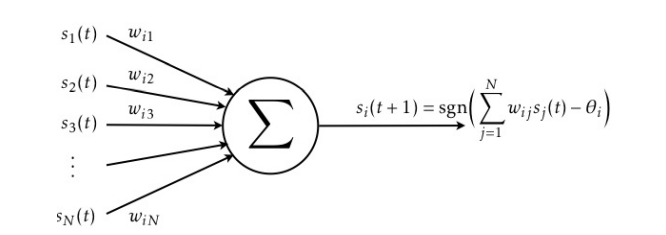
\includegraphics[width=0.5\textwidth]{Figures/neuron.PNG}
  \caption{\small{Schema di un percettrone. ~\cite{reti}
   } % end small
  } % end caption
  \label{fi:dcalc}
\end{figure}
La somma pesata e shiftata viene poi passata per una determinata funzione \emph{f}, 
che nel caso del neurone di McCulloch e Pitts  è la funzione segno \emph{sgn()}.\\
Nel deep learning la funzione segno è molto spesso sostituita da una funzione f chiamata
 \emph{funzione di attivazione}. La funzione di attivazione definisce l’uscita di un neurone 
 in funzione del suo livello di attivazione \(b_i(t)\).
Una scelta comunemente utilizzata è la \emph{sigmoide}: 
\[f(x)= \frac{1}{1+\mathrm{e}^{-x}}\]
Un’altra molto importante e anch’essa utilizzata è la \emph{ReLU} (Rectified Linear Unit):
\[f(x) = x^{+} = max(0,x)\]

Tale funzione è una di quelle maggiormente impiegaye negli algoritmi di deep learning per la rapidità di 
apprendimento che permette di sviluppare nelle reti formate da vari strati di neuroni 
e per altri fattori che saranno approfonditi in seguito. \\
La formula (2.1) è anche la formula che definisce la \emph{regressione logistica}, l’algoritmo d’apprendimento base di cui si compongono le
reti neurali.
La computazione fatta nel singolo neurone viene poi eseguita in maniera parallela per tutti 
i neuroni e gli output di \(s_i\) diventano gli input per i neuroni dello strato successivo a quello
 i-esimo. Lo scopo quindi di Mc-Culloghs è stato quello di costruire un modello che simulasse le dinamiche 
 delle reti neurali reali.\\
 \begin{figure}[hb!]
  \centering
  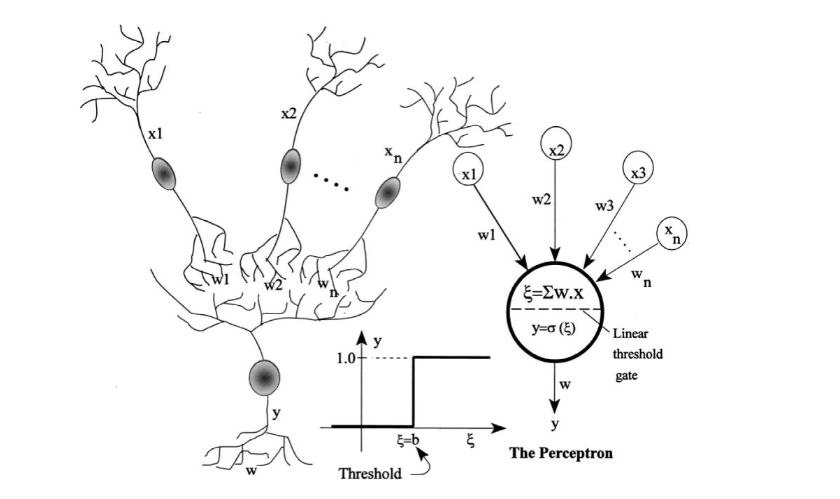
\includegraphics[width=0.8\textwidth]{Figures/confronto neurone biologico-artificiale.PNG}
  \caption{\small{Figura che rappresenta come le reti neurali siano effettivamente ispirate alle reti neurali biologiche. A sinistra vi è una rete di neuroni reali e a destra un modello di percettrone.
  } % end small
  } % end caption
  \label{fi:dcalc}
\end{figure}

Dato che una rete neurale efficiente deve essere in grado di apprendere e fornire uscite a fronte di 
input anche sconosciuti, occorre allenare la rete con degli algoritmi. 
L’addestramento della rete neurale si basa sulla presentazione al suo ingresso di una serie di esempi,
 la cui natura la rete è in grado di riconoscere, che costituiscono il dataset di training. 
 Le risposte che la rete fornisce vengono confrontate con quelle attese e si calcola l’errore tra le due.
  Sulla base di tale errore i pesi vengono modificati istante per istante, e la procedura viene ripetuta
   fino a che la rete non fornisce un errore che sia al di sotto di una determinata soglia prestabilita.
     


Una rete neurale di dice stratificata quando è formata da vari strati di neuroni, 
tali che ognuno di loro sia connesso con quelli dello strato successivo, ma senza che ci 
siano connessioni tra neuroni del medesimo strato. 
Il neurone pensato da Mc-Culloghs è chiamato anche Percettrone e possiede solamente uno strato di input e uno di output.
Di solito si lavora con reti in cui vi sono uno o più \emph{hidden layers}, 
i quali non comunicano direttamente con l’esterno. Queste reti sono chiamate MPL (Multi-Layer-Perceptron). 

Il primo vero miglioramento rispetto al Perceptron è stato l’\emph{Adaline} (ADAptive LInear NEuron), 
in quanto utilizza proprio una funzione di attivazione lineare per regolare il vettore 
dei pesi al posto della funzione a gradino. \\


Una rete neurale artificiale in cui per ogni strato il segnale di ingresso viaggia
sempre in avanti dall’ingresso all’uscita, senza creazione di cicli, si chiama \emph{feedforward}. \\




L'\emph{apprendimento profondo}~\cite{dl}, in inglese Deep Learning (DL) è quel campo di ricerca del ML 
e dell'Intelligenza Artificiale che studia le tecniche e i sistemi per consentire alle macchine 
di apprendere in autonomia in modo profondo. Nello specifico, questa branca viene considerata una
 categoria sottostante al machine learning, in quanto si tratta di un approccio per l’apprendimento
  automatico dei sistemi informatici. \\
  In altre parole, per apprendimento profondo
   si intende un insieme
   di tecniche basate su reti neurali artificiali organizzate in diversi strati, dove ogni strato calcola
    i valori per quello successivo affinché l'informazione venga elaborata in maniera sempre più completa
     con l’aumentare della profondità. Lo sviluppo del deep learning è motivato in parte dal fallimento
      degli algoritmi
      tradizionali di ML nel tentare di svolgere compiti delle AI, come ad esempio speech recognition e object recognition. 
      Il principio di funzionamento è lo stesso delle reti neurali classiche, con una differenza
       che risiede nel numero molto elevato di livelli nascosti di neuroni intermedi.
       Altre sfide che hanno portato allo sviluppo dell’apprendimento approfondito è la difficoltà
       degli algoritmi classici nel generalizzare su problemi con dati multi-dimensionali.
       Il fenomeno legato alla grande dimensionalità dei dati è conosciuto come \emph{course of 
       dimensionality}~\cite{dim}: questo fenomeno si presenta spesso in molti campi della computer science,
        in particolare nel machine learning. É stato introdotto questo problema per la prima volta
         dal matematico Richard Bellman e indica che il numero di campioni necessari per
          stimare una funzione arbitraria con un dato livello di accuratezza
           cresce esponenzialmente rispetto al numero di variabili di input
            (cioè dimensionalità) della funzione.
             
    \begin{figure}[H]
      \centering
      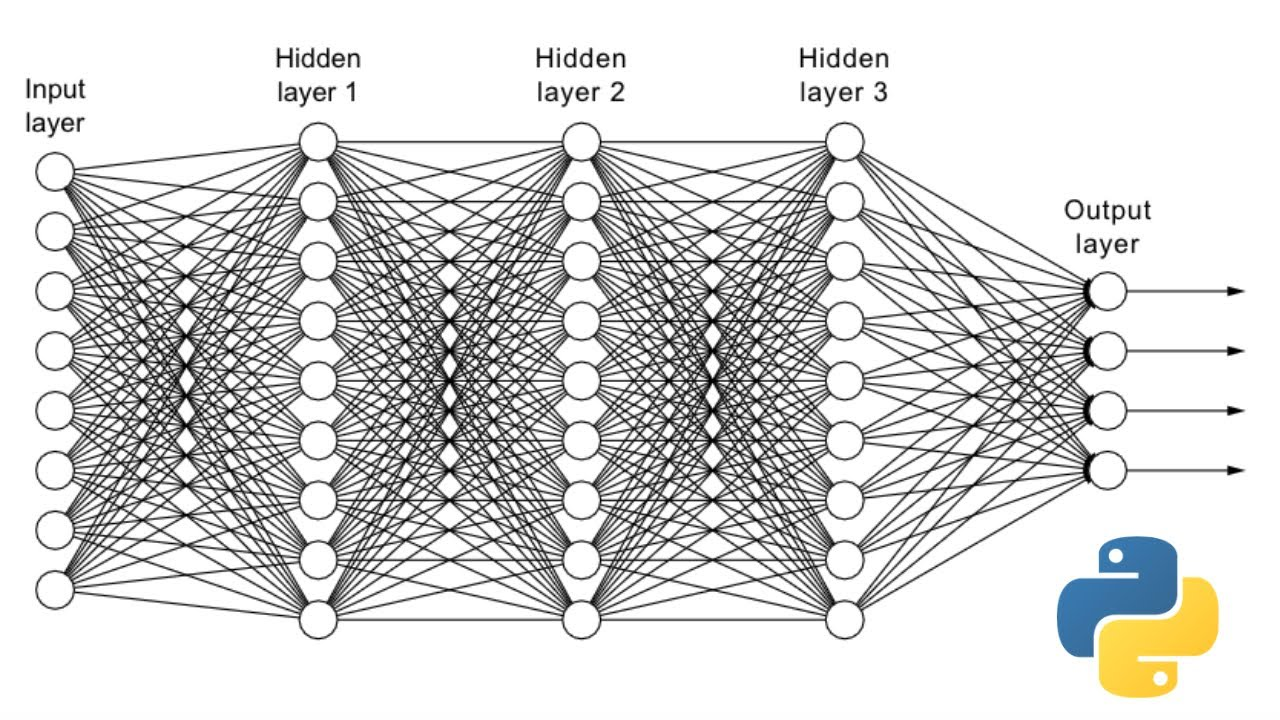
\includegraphics[width=0.8\textwidth]{Figures/deep-neural-network.jpg}
      \caption{\small{Esempio di rete neurale profonda con 3 strati nascosti.~\cite{dnn}} % end small
      } % end caption
      \label{fi:dcalc}
    \end{figure}
    
       All’aumentare del numero dei dati aumenta anche il numero delle \emph{features} (cioè il numero di parametri con cui i dati possono essere descritti),
        ma
        all’aumentare delle features diminuisce anche la capacità predittiva del
       sistema con un conseguente peggioramento delle prestazioni.
       Come già detto nel precedente capitolo, con i metodi convenzionali di machine learning
       bisogna costruire gli estrattori delle feature dei dati di input. L’accuratezza e la precisione
       delle predizioni sono fortemente influenzate dall’abilità di colui che realizza il modulo di
       estrazione, che richiede inoltre un forte sforzo ingegneristico.\\
       Un vantaggio fondamentale delle reti di deep learning è la possibilità di migliorare le prestazioni 
       con l’aumentare del formato dei dati.

Un’organizzazione gerarchica dei dati permette di condividere e riutilizzare informazioni
 estratte durante l’elaborazione e di selezionare e scartare dettagli inutili lungo una gerarchia.
  Rispetto ad una architettura semplice a tre strati (input-strato con unità nascoste-output),
   una architettura multi-strato permette di distribuire meglio un grande numero di nodi 
   su più livelli riducendo il costo computazionale elevato che si avrebbe se i nodi fossero
    tutti localizzati
    su uno soloe attenuando l’ingente utilizzo di memoria che comporterebbe una 
    struttura meno profonda. \\ 
    In generale le tecniche di deep learning stanno diventando sempre più utili anche in quello
     che è il campo della \emph{computer vision}, 
    cioè l'area di studio delle AI che si occupa della ricerca sull'automatizzazione 
    dell'informazione visuale, e in particolare anche dell'analisi di dati biomedici,
     come nel caso del presente lavoro di tesi.\\
    
      
     Le Deep Feedforward Networks~\cite{tesi}, chiamate anche multilayer perceptrons (MLPs), 
     sono degli strumenti molto importanti usati nel DL.
     L’obiettivo delle MLPs è approssimare una funzione $f^{*}$. 
     Ad esempio, se si vuol costruire un classificatore si esegue una mappatura
     dell’input x su una categoria y: y = $f^{*}(x)$ . Una rete di tipo feedforward definisce una mappatura 
     y = f (x, \(\theta\)) e cerca il parametro \(\theta\) che renda migliore l’approssimazione
      della funzione.
     Questi modelli sono chiamati feedforward perché l’informazione fluisce prima attraverso
     la funzione che deve valutare \emph{x}, poi lungo le elaborazioni intermedie usate per definire \emph{f}
     fino all’output y. 
     Questo tipo di reti sono di solito rappresentate dalla composizione di più funzioni ad
esempio $f^{1}$, $f^{2}$ e $f^{3}$ connesse da una catena:
 $$f(x) = f^{3}(f^{2}(f^{1}(x)))$$
n questo caso $f^{1}$ sarà chiamato primo strato (first layer), $f^{2}$ secondo strato e così via.
La lunghezza della catena indica la \emph{profondità} del modello. Lo strato finale della rete è
chiamato strato di output. \\
Durante l’addestramento della rete si cerca di approssimare 
$f (x)$ ad una funzione $f^{*}(x)$ valutata su differenti esempi di addestramento. \\
Questi specificano direttamente cosa deve fare lo strato
di output ad ogni punto \emph{x}: deve produrre un valore il più vicino possibile alla label di target y. \\
Il 
comportamento degli altri strati non è direttamente specificato dai dati di addestramento;
l’algoritmo di apprendimento deve decidere come usarli per produrre l’output desiderato
per implementare al meglio una approssimazione di $f^{*}$. Siccome i dati di addestramento 
non mostrano l’output desiderato per ognuno di questi strati vengono chiamati \emph{strati
nascosti}. La dimensione degli strati nascosti determina la larghezza del modello.\\
Lo strato rappresenta una funzione a valori vettoriali formata da molte \emph{unità} che agiscono in
parallelo, ognuna rappresentante una funzione a valori vettoriali che restituisce un valore
scalare. Ogni unità è assimilabile ad un neurone nel senso che essa riceve l’input da altre
unità ed elabora un output che verrà mandato a sua volta come input ad altre unità. Il
valore di output viene chiamato valore di attivazione, che è analogo a quello delle reti neurali non profonde. 
\section{Addestramento di una rete}

Come è stato già detto in precedenza, il punto di partenza per l’addestramento in generale, ma ancora di più per addestrare una rete neurale, 
è avere a disposizione un dataset formato da un insieme di training che verrà somministrato in
 input alla rete per estrarne automaticamente le features, e un insieme di test con dati completamente nuovi al sistema
  per verificare l'efficacia dell’addestramento stesso. \\
  Per semplicità, assumiamo che il problema che vogliamo risolvere sia un problema di classificazione binaria. Per esempio vogliamo decidere se, data una certa
immagine, questa rappresenti o meno un gatto.\\
Rappresentiamo la nostra immagine come un vettore x unidimensionale di byte.
Fissiamo y = 1 nel caso in cui l’immagine rappresenti un gatto, y = 0 nel caso in
cui nell’immagine non ci sia un gatto. La nostra unità di regressione logistica dovrà
dunque calcolare un’approssimazione di y; più precisamente calcolerà le probabilità
che nell’immagine ci sia un gatto.
Dato x, vogliamo dunque calcolare l'approssimazione 
$\hat{y}$ = P(y = 1$\mid$x). 
Perché ciò avvenga, serve che i parametri \emph{w} e \(\theta\) siano opportunamente configurati, 
ed è qui che entra in gioco il concetto di apprendimento.
  Durante l’addestramento, dopo aver fornito l'input,
   la rete produce un output in forma di
vettore di risultati. Bisogna calcolare una funzione che misuri l’errore (o la distanza) tra i
 risultati di output e i risultati desiderati, cioè i valori con cui vengono etichettati i 
 dati nell’apprendimento supervisionato.\\
  La funzione che ci permette di farlo è chiamata \emph{funzione di errore} o di perdita.
   Una delle funzioni di errore utilizzata nell’apprendimento supervisionato è la MSE 
   (Mean Squared Error):
   \begin{equation} \label{2}
MSE = \frac{1}{2}\sum (out - target)^{2}
   \end{equation}
 Nel deep leaning è molto utilizzata \emph{funzione di entropia incrociata}, 
funzione di perdita che serve per quantificare la differenza tra due distribuzioni di 
probabilità:
 quella che vorremmo il nostro sistema raggiungesse, e quella che il nostro sistema ha elaborato statisticamente
 fino a quel momento. Viene descritta dalla seguente formula:
 \[ H(h,q) = -\sum_{x}^{}p(x) \log (q(x))\] 
 dove \emph{p} è la funzione di distribuzione da raggiungere su un insieme di eventi \emph{x}, mentre \emph{q} 
 è quella fino ad ora elaborata. 
 Ogni volta questa funzione ci indica quanto la nostra stima fatta si discosti dalla realtà.\\

La rete in fase di addestramento modifica i suoi parametri interni variabili in modo da
 minimizzare la funzione di costo. Questi parametri sono chiamati pesi e spesso sono numeri 
 reali che possono essere visti come delle "manopole" che definiscono la funzione di input-output
  della rete.
Per modificare in maniera appropriata il vettore dei pesi, l’algoritmo di apprendimento calcola 
un vettore gradiente che, per ogni peso, indica di quanto l’errore cresce o decresce se 
i pesi vengono incrementati di una quantità infinitesima. Il vettore gradiente,
 calcolato sulla funzione di costo indica la direzione più ripida e 
 veloce su come andare a aggiornare i pesi stessi, portandosi sempre più vicino a dove
l’errore di stima dell'output è minore in media.\\
L’approccio più utilizzato al fine di minimizzare l’errore è la procedura chiamata \emph{gradiente stocastico 
decrescente}~\cite{ann}. Esso consiste nel mandare in input alla rete alcuni esempi,
calcolandone l’output con la (2.1), l’errore associato (ad esempio con la (2.1)) e il gradiente medio
di questa ultima variando i pesi in maniera infinitesima. La procedura è
iterata per molti set piccoli di esempi presi dall’insieme di addestramento finchè la media
della funzione oggetto non smette di decrescere. Si parla di gradiente stocastico perchè ogni piccolo
 insieme di esempi fornisce una stima del gradiente medio su tutti gli altri.\\
A titolo di esempio, si mostra successivamente come funziona l’algoritmo del gradiente discendente 
per un semplice percettrone. 
\begin{enumerate}
\item La rete prende in ingresso dei valori randomici iniziali per i pesi W e un valore costante,
 il learning rate \(\eta\). Tale valore determina lo step da fare ad 
 ogni iterazione nella direzione indicata dal gradiente. 
\item Si calcola la funzione di costo con i parametri attuali;
\item Si aggiornano i valori dei pesi usando la funzione di aggiornamento dei pesi W che è:
 \begin{equation} \label{3}
W^{(\rho)} = W^{(\rho -1)} - \eta \frac{\partial E}{\partial W}
\end{equation}
dove \(\rho\) indica il valore dei pesi al passo precedente e \(\eta\) il learning rate.
\item Alla fine l'algoritmo ritorna il costo minimizzato per la funzione di errore. \\

Occorre dunque vedere come il valore dei pesi ha effetto sulla funzione di errore.
 Si applica la regola della catena di derivazione:\\

\[\frac{\partial E}{\partial W}  = \frac{\partial E}{\partial out}  \frac{\partial out}{\partial in}  \frac{\partial in}{\partial W} \] \\

dove \emph{in} è la funzione che è combinazione lineare di input e pesi, 
mentre \emph{out} è l’output che si ottiene facendo passare \emph{in} per la funzione di attivazione,
 per esempio la sigmoide.
Nel caso in cui si abbia una rete senza hidden layers la regola della catena si applica nel modo seguente, 
se vi fossero più strati però la procedura è analoga andando ad applicare tale regola
 per ognuno degli strati. 
Se si vanno a valutare le nostre derivate per il caso del percettrone, si può facilmente dimostrare che:\\
\[\frac{\partial E}{\partial out} = (out - target),\]
\[\frac{\partial out}{\partial in} = out(1-out),\]
\[\frac{\partial in}{\partial W} = in \]
Si moltiplicano tra loro dunque tutti i termini derivativi e poi si applicano all’equazione principale (2.3) 
e si aggiornano i valori dei pesi di conseguenza, fintanto che la media dell’errore non converge, ovvero smette
 di decrescere. 
\end{enumerate}
Tale algoritmo nelle prove sperimentali ha effettiva realizzazione in quello che è chiamato l’\emph{ottimizzatore}
 (uno dei più è efficienti è proprio SGD (Stochastic Gradient Descent), ma vi sono anche Adam, ADAline... 
 Tutti però seguono l’idea di base del gradiente discendente.\\ 
 Infine terminata questa procedura si passa alle valutazioni sulla performance della rete;
  essa viene misurata con gli esempi dell’insieme di test.\\
 Il metodo migliore per minimizzare la funzione di errore è proprio quello di usare il gradiente.
 Nelle reti MLP (Multi-Layer-Perceptron) si effettuano una serie di derivate successive e
  ogni volta si trova il punto che annulla la derivata della funzione di errore. Questo procedimento è 
  piuttosto semplice nelle reti neurali più basilari, mentre inizia ad essere più complicato
   nelle reti neurali con più strati perchè vi possono essere più minimi locali. In questo caso si gioca sul valore del learning rate.
   Un valore del learning rate (di solito compreso tra 0 e 1) troppo alto farà fare un
    salto troppo grande verso il minimo della funzione di costo, 
   facendo perdere alla rete capacità di convergenza (rischiando in alcuni casi anche la divergenza) mentre un learning rate troppo basso rallenta
    notevolmente il training e può comportare il fatto che l'algoritmo rimanga fermo nel 
    calcolo di un minimo locale indesiderato per la funzione di errore. \\
   

Dunque, il ciclo di apprendimento di una rete neurale feedforward può essere sintetizzato in due fasi:
\begin{itemize}
\item fase di FEEDFORWARD: si fanno passare i pattern dei dati di addestramento (input features) 
attraverso la rete per ottenere un output;\\
\item fase di BACKPROPAGATION: si calcola la differenza tra l'output e il valore di
  target (di base si calcola l’errore di predizione) e si utilizza così l’algoritmo Gradient Descent 
  per aggiornare i valori dei pesi. In pratica si riporta il valore dell’errore all’ingresso, 
  ne si calcola la sua derivata rispetto ad ogni peso della rete e ogni volta si aggiornano i
   valori dei pesi del modello. 
\end{itemize}
 Dopo varie iterazioni dei due passi si ottiene una maggiore accuratezza di predizione per la rete. \\ 
 Nelle reti neurali profonde si utilizzano gli algoritmi di 
 back-propagation per facilitare il procedimento di calcolo del gradiente. In questi algoritmi
  i pesi sono calcolati partendo dall’ultimo strato di neuroni procedendo all’indietro.
   Un ciclo di presentazione alla rete di tutti gli eventi appartenenti all’insieme di 
   addestramento è detto \emph{epoca}. \\
 
 La procedura di propagazione all’indietro calcola il gradiente di una funzione oggetto
  in funzione dei pesi associati ai propri parametri proprio applicando semplicemente 
  la regola di derivazione della catena: la derivata, o proprio il gradiente, di una 
  funzione rispetto ai valori di input può essere calcolata propagando all’indietro,
   dall’output del modello fino ad arrivare al primo strato. 
   Partendo dall’output, cioè lo strato dove la rete produce le sue predizioni,
    il gradiente fluisce attraverso tutto il modello fino ad arrivare all’input, 
    dove sono forniti i dati su cui sono fatte le predizioni.\\
     Una volta calcolati questi gradienti è facile trovarne l’espressione
      dipendente dai pesi associati ai parametri della funzione oggetto.\\
    


 
\section{Overfitting e underfitting}
L’abilità di un algoritmo di performare bene su input mai osservati precedentemente si chiama
 generalizzazione. Un buon algoritmo di machine learning è un algoritmo che possiede errore 
 di generalizzazione minimo. \\
I termini \emph{overfitting} e \emph{underfitting} sono nati proprio come risposta alle deficienze di cui 
il modello può soffrire. Pertanto sapere quanto il modello commette errori, significa sapere
 quanto questo va in overfitting o underfitting. 
Come è possibile influenzare l’errore sull’insieme di test quando 
questo insieme non si conosce a priori?\\
 Il campo della teoria dell’apprendimento statistico fornisce 
alcune risposte. Attraverso delle assunzioni riguardanti la maniera in cui sono stati raccolti
 i dati si possono studiare matematicamente le relazioni che intercorrono tra l’errore dell’insieme
  di addestramento e l’errore sull’insieme del test.

Quindi, dopo aver generato l’insieme di addestramento, si scelgono e si variano i parametri per
 ridurre l’errore sull’insieme, che dovrebbe corrispondere anche all’errore sull’insieme di test.
I fattori che determinano quanto sia efficiente un algoritmo di apprendimento sono:
\begin{enumerate}
  \item la sua abilità nel minimizzare l’errore di addestramento;
  \item la sua abilità nel minimizzare il gap tra errore di addestramento e l’errore di test.\\
\end{enumerate}
L’\textbf{underfitting} è quando il modello non riesce a rendere l’errore di addestramento
 sufficientemente piccolo. Questo significa che il modello è troppo semplice e non si 
 riescono a identificare un numero sufficiente di features, il che rende impossibile al 
 modello di apprendere da quel dataset. In termini di machine learning significa che c’è 
 stato un focus troppo basso sul set di training, dunque il modello non è nemmeno in grado
  di testare correttamente.
L’\textbf{overfitting} è il caso in cui il modello ha imparato molto bene dal suo dataset di training,
 ma non è in grado di generalizzare bene. Questo significa che c’è un forte gap tra errore 
 di addestramento ed errore di test. In termini di machine learning vuol dire che che c’è
  stato un eccessivo focus nel training set, e che le relazioni stabilite tra i neuroni
   non sono valide per valutare correttamente nuovi dati.  
Generalmente gli algoritmi di machine learning performano meglio quando la capacità dei dati 
è appropriata per la reale complessità del compito che devono svolgere e la quantità di dati 
dell’insieme di addestramento forniti. Modelli con capacità insufficiente non sono capaci di
 svolgere compiti complessi. Modelli con grande capacità possono risolvere compiti difficili,
  ma nel caso in cui la capacità sia più grande di quella richiesta del compito da svolgere
   potrebbero andare in overfitting.
In effetti nel machine learning i modelli sono soggetti al problema del \emph{trade-off varianza-bias}.
 Questo nasce come conflitto nel provare a minimizzare simultaneamente le due fonti di errore che 
 impediscono al modello di generalizzare:
 \begin{itemize}
     \item errore di bias, che è consequenziale ad errate assunzioni fatte dall’algoritmo di learning, 
per rendere il dataset più facilmente allenabile (underfitting).
\item errore di varianza, dato dalla forte sensitività del modello a fronte di piccoli cambiamenti 
del training set, con conseguente aumento di rumore (overfitting). 
\end{itemize}

É impossibile minimizzare entrambe, ma è possibile raggiungere un buon compromesso tra le due. \\

Un modo per evitare underfitting (bias alto) è quello di utilizzare una maggior quantità di 
dati ma questo non sempre funziona. Altrimenti si può incrementare la complessità del modello, 
riducendo il rumore dei dati oppure aumentando il numero di epochs e quindi incrementando la
 durata del training. \\
Tutto ciò però nella misura tale per cui non si ricada nell’overfitting (alta varianza), 
che può essere evitato ad esempio riducendo la complessità del modello, in quanto dati
 troppo ‘rumorosi’ possono portare a valutazioni erronee e poco generalizzabili. Un altro
  modo è quello di ridurre il numero di parametri o come si vedrà in seguito nelle CNN, usando dei Dropout.
   Un’altra tecnica è quella di utilizzare alcune funzioni, come EarlyStopping in Keras che
    valutano passo passo l’andamento del training e lo fermano non appena si nota che 
    il modello non è più in grado di generalizzare, cioè prima che cada in overfitting.\\
    Si andrà più nel dettaglio di Keras e delle sue funzioni in seguito (sez. 4).
   
    \begin{figure}[H]
      \centering
      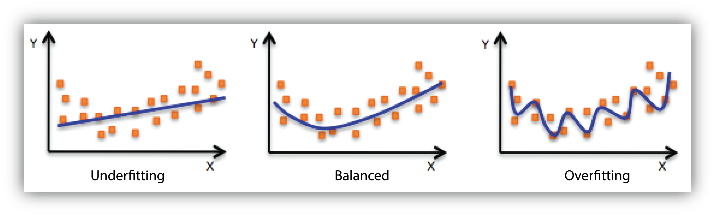
\includegraphics[width=0.8\textwidth]{Figures/ofuf.PNG}
      \caption{\small{I grafici mostrano cosa significa underfitting e overfitting in maniera visiva.~\cite{ofuf} Si può vedere
       come la prima curva di regressione non vada a suddividere in maniera precisa i dati in rosso, mentre l'ultima curva separi bene tutti i dati classificandoli, ma è una curva troppo precisa e specifica per i dati di interesse e che probabilmente non andrà a dare risultati corretti se i dati in ingresso si discostano anche leggermente da quelli rossi in figura. Al centro invece la curva risulta essere bilanciata. 
      } % end small
      } % end caption
      \label{fi:dcalc}
    \end{figure}
    
% end caption
     

\section{Classificazione}
Come detto in precedenza, in questo lavoro di tesi le reti saranno addestrate al fine 
della classificazione  ~\cite{classdef} delle immagini di raggi-X pettorali in una prima esperienza e altre immagini
 di risonanza magnetica cerebrale in una seconda
esperienza. 
Riuscire ad estrarre informazioni utili dalle immagini non è affatto facile e spesso 
la possibilità di codificare al meglio l’informazione è inibita da fattori quali un errore 
sul modello o una scorretta acquisizione dell’immagine. Ciò che permette di estrarre le 
informazioni dalle immagini sono le feature delle stesse, identificando oggetti nell’immagine
 che risultano avere caratteristiche comuni. Schemi ricorrenti nei soggetti malati (o anche
  nei soggetti sani) permettono di sviluppare criteri oggettivi per determinare la diagnosi 
  dei pazienti ricercando tali schemi.\\
   Come nel caso del dataset del Brain Tumor utilizzato 
  nella tesi, nelle diverse categorie di tumore è sicuramente necessario riconoscere l’adenoma 
  a seconda della sua forma e della variazione di colorazione con cui la massa tumorale si presenta.
   Dal riconoscimento di determinate
   caratteristiche è possibile classificare un oggetto mai visto prima dal sistema attribuendogli
    un classe di appartenenza o label definita a priori.
In questo lavoro di tesi il processo di classificazione si è basato su un approccio supervisionato
 definito nel paragrafo 2.1. Occorre andare ad estrarre all’oggetto in esame, 
 nel nostro caso a immagini di risonanze magnetiche, un certo numero di caratteristiche 
 che ci permettano di identificarlo e la rete neurale utilizzata andrà a farlo direttamente da sola.\\
 Nei problemi di classificazione 
supervisionata come quello di interesse occorre costruire un classificatore in grado di 
apprendere dai dati in ingresso e riuscire così a classificare anche un dato mai visto e
 del quale si vuol conoscere la classe di appartenenza. 
Lo scopo principale delle nostre reti usate per la classificazione mediante un approccio 
di apprendimento supervisionato è quello di definire delle buone regole di decisione per
 l’assegnazione delle etichette ad oggetti sconosciuti, sulla base delle conoscenze che 
 il modello ha acquisito. Per una generica osservazione y, ed un numero di classi k, il 
 classificatore può essere definito dalla funzione:
\[C(y) : R^{n} \rightarrow 1 … k\] 
Se y appartiene alla classe j e C(y) \(\neq\) j, si dice che il classificatore C commette un errore
nella classificazione di y. Chiamati I l’insieme dei dati di input e O l’insieme dei dati
 di output, si definisce una funzione h tale che associ ad ogni dato di ingresso I la sua 
 risposta corretta. Questa funzione h non si conosce ed è quella che va appresa.
  L’accuratezza di un classificatore C indica la porzione di elementi correttamente 
  classificati su un gruppo di dati \(N_t\) con classe nota rapportata ai totali classificati. 
  Dunque la porzione di dati non correttamente classificati sarà: \( \delta E = \frac{N_{err}}{N_t}\).

Abbiamo quindi descritto le reti neurali come una semplice catena di strati caratterizzata
 dalla profondità del modello e dalla larghezza di ogni strato. Variando questi parametri 
 si possono ottenere un numero considerevole di architetture diverse. Molte architetture
  sono state sviluppate per compiti specifici e nel presente lavoro di tesi saranno approfondite
   quelle che sono state utilizzate nella fase sperimentale per la classificazione:
    le CNN (Convolutional Neural Networks). 
Nel capitolo successivo viene una piccola digressione su modello matematico di tali reti.



